 \documentclass[9pt, onecolumn,twoside]{gsajnl}
% how i want it for inport into word: \documentclass[9pt, onecolumn,twoside]{gsajnl}
% how i want it for pdf: \documentclass[9pt,twocolumn,twoside,lineno]{gsajnl}
% Use the documentclass option 'lineno' to view line numbers

\usepackage{epstopdf}
\usepackage[T1]{fontenc}
\usepackage[latin1]{inputenc}
\articletype{inv}
\runningtitle{Soy scientific manuscript} % For use in the footer
\runningauthor{Connelly \textit{et al.}}

\title{SoyAdapt}

\author[1,$\ast$]{Josephine Estelle Ananda Connelly}
\author[2,$\dagger$]{Guillaume Paul Ramstein}
\author[3,$\dagger$]{Wolf L Eiserhardt}
\author[4,$\dagger$]{Torben Asp}


\affil[1,2,4]{Centre for Quantitative Genetics and Genomics, Faculty of Technical Sciences, Aarhus University (DK).}
\affil[1,3]{Department of Biology, Faculty of Natural Sciences, Aarhus University, (DK).}
\affil[3]{Royal Botanic Gardens, Kew, (UK).}

\affil[$\dagger$]{These authors share senior authorship}
\correspondingauthoraffiliation[$\ast$]{Corresponding author: AU, josephineconnelly@qgg.au.dk.}

\begin{abstract}
Soybean (Glycine max L. Merrill) is the worlds leading  oilseed crop used as a  primary source of vegetable oil for human consumption and in protein meal for animal feed.

Search engine optimization (SEO)

There are a few simple ways to maximize your article's discoverability and search results.

    Include a few of your article's keywords in the title of the article

    Do not use long article titles

    Pick 5-8 keywords using a mix of generic and more specific terms on the article subject(s)

    Use the maximum amount of keywords in the first two sentences of the abstract

    Use some of the keywords in level 1 headings

    Title

The title should be concise, omitting terms that are implicit and, where possible, be a statement of the main result or conclusion presented in the manuscript. Abbreviations should be avoided within the title.

Witty or creative titles are welcome, but only if relevant and within measure. Consider if a title meant to be thought-provoking might be misinterpreted as offensive or alarming. In extreme cases, the editorial office may veto a title and propose an alternative.

Authors should avoid:

    titles that are a mere question without giving the answer

    unambitious titles, for example starting with 'Towards,' 'A description of,' 'A characterization of' or 'Preliminary study on'

    vague titles, for example starting with 'Role of', 'Link between', or 'Effect of' that do not specify the role, link, or effect

    including terms that are out of place, for example, the taxonomic affiliation apart from species name.

For Corrigenda, General Commentaries, and Editorials, the title of your manuscript should have the following format.

    'Corrigendum: [Title of original article]'

    General Commentaries:
    'Commentary: [Title of original article]'
    'Response: Commentary: [Title of original article]'

    'Editorial: [Title of Research Topic]'
\end{abstract}

\keywords{Soy; population genetics; Diversity; Selection; more keywords}

\dates{\rec{01 09, 2023} \acc{01 09, 2023}}

\begin{document}

\maketitle
\thispagestyle{firststyle}
\vspace{-13pt}

\section{Introduction}

\textit{what we already know:} Several severe genetic bottlenecks occurred in soybean. Compared to the wild species, the genetic diversity was halved, resulting in a loss of 81\% of rare alleles (Hyten et al., 2006). Additionally, two major bottlenecks occurred during the development of North American modern cultivars, where only a few landraces were used. And as a result of intensive soybean breeding over the past 75 years. Elite cultivars have emerged, but they are derived from only about 19 landraces. Consequently, the North American breeding pools now retain only 72\% of genome diversity and have lost 79\% of rare alleles found in diverse landraces (Gizlice et al., 1996).

\textit{soybean needs to be grown in the north}:
Modern soybean breeding has led to yield increases of $229 \, \text{kg} \, ha^{-1} \, \text{yr}^{-1}$ (Rincker et al., 2014), gaining a deeper understanding of the genomic basis of this progress could offer valuable insights for advancing and adapting soybean cultivation even further.

Expanding the production of soy to the northern climates by leveraging the advancements in soybean breeding and focusing on the genes relevant to adaption, can diversify the global supply chain, reduce dependency, and potentially alleviate the environmental pressures associated with soy production in high biodiversity, sensitive areas/ecologically vulnerable regions. With the global demand for soy and the need for sustainable agricultural practices, investing in breeding programs to develop soybean varieties suitable for northern climates can present a promising solution. 




 
\textit{the Swedish soybeans (goals and scope)}

\textit{mention approaches}

\textit{In this study we}
The goal is to help precipitate the utilisation of these soybean genetic resources. to increase germplasm utilization for through understanding what we have in the genebanks. 

\section{Materials and methods}
\label{sec:materials:methods}

\subsection{Swedish Breeding Program Collection}
155 soybean accessions were obtained from the Nordgen genebank of Swedish origin. These accessions originate from a Swedish breeding program (SBP) running from the 1840s to the 1970s which used material consisting of a mixture of elite cultivars of the time and Japanese landraces, breeding for the adaptation to the cool climate of northwestern Europe \cite{holmberg1973}. 

\subsection{The Core Collection}
The Core Collection (CCA) consists of two samplings of the core collection from haupt20. A 5\% and 10\% collection with overlapping accessions in total consisting of 409 accessions after filtering. 
The Core collection accessions (CCA) used here is a subset of the large soybean germplasm collection, the  USDA genebank accessions consisting of 415 of the USDA soy germplasm accessions. This Core collection has been selected with a focus on adaptation to high-latitude cold regions using environmental data from phenotypic trials in Germany, and comparing Donor opulation of Environments (DPE) in Asia and the Target Population of Environments (TPE) in Central Europe by \cite{haupt20}. From the more than 17.000 accessions, two diverse core collections of 183 and 366 accessions were created. These 514 diversity panels are used here due to that they are likely preadapted to cultivation in Central Europe, while simultaneously conserving a high level of genetic diversity. 

\subsection{The Founders Collection}
The USDA Soybean Germplasm Collection maintains accessions of >17000 cultivated soybeans and is part of the U.S. National Plant Germplasm System (NPGS).  These accessions have been previously genotyped with the SoySNP50K iSelect BeadChip  \cite{song13,song15} has been used for genotyping the USDA Soybean Germplasm Collection and is available for use from SoyBase (https://soybase.org/) in the version mapped to the soybean genome assembly Glyma.Wm82.a2  \cite{schmutz10}. In the pedigree information from Nordgen SBPA, are 10 accessions present in the USDA genebank and thus are part of the SoySNP50K genotypic data. These specific accessions were included as they are considered Founders of the SBP. 

\textit{DNA extraction and sequencing information?:}

\subsection{Genotyping and filtering of whole genome sequence SNP}
The accessions from the Nordgen genebank and the Core collection accessions were whole genome sequenced. Four of the Core collection seeds didn't germinate in time for the sequencing, resulting in accessions sequenced 574. Of the Nordgen accessions, Four were of Latvian origin and therefore excluded in further analysis. 
The reads were aligned to the Williams 82 2a reference genome \cite{schmutz10} using an adapted GATK Best Practices \cite{mckenna10}, keeping MQ30 and biallelic sites and using VCFTools \cite{danecek11} applying a minor allele frequency (MAF) filter of 0.01 in order to remove rare variants from the data, reducing the number of SNPs markers were initially called (raw dataset) from 17,648,123 to 10,000,122. 
For a detailed account of accessions, programs and commands used see supplementary material: \nameref{sec:supplementary:material} 
A further three accessions were removed due to missing phenotype data and a single accession that had missing data > 5$\%$ using BCFtools \cite{danecek21}, resulting in 153 Swedish accessions from the NordGen genebank and 409 of the CCA accessions. Five per cent missing data at SNPs was also removed resulting in an SNP count of 8,533,444. This data set was used to compare the Allele Frequency of the two populations. For all other analyses, MAF 5\%  was removed using Vcftools (--maf 0.05) on the dataset as a whole, except for the case of LD calculation MAF5\% was removed separately for SBPA and CCA.  

\subsection{SNP intersect }
An intersection was made of the whole genome sequenced data (153 SBPA and 409 CCA) and the SoySNP50K array data of the 10 Founders.  This was done using BCFtools with the command "isec". The intersecting data was 35.486 SNPs. 

For a detailed account of programs and commands, see supplementary material, \nameref{sec:supplementary:material} (S3: Methods 1) data preparation and filtering and \nameref{sec:data:availability} for data. 

\subsection{Population Structure Analysis}
To infer population stratification of the Swedish accessions from the NordGen gene bank and the Core collection and of the 12 accessions assumed to be founders of the Swedish breeding program. Principal component analysis (PCA) on SNP genotype data was applied using the package SnpRelate in R (A Parallel Computing Toolset for Relatedness and Principal Component Analysis of SNP Data). The functions in SNPRelate for PCA used (snpgdsPCA) calculate the genetic covariance matrix from genotypes, computing the correlation coefficients between sample loadings and genotypes for each SNP and SNP eigenvectors were calculated. The WGS data was used for a number of the PCA, and where the possible genetic Founders to the Swedish breeding program the intersect data is used and indicated in figures; \ref{fig:pca}.

The package SNPRelate in R was used to compute an identity-by-state (IBS) matrix that calculates the proportion that two randomly selected reads that contain a certain SNP locus are the same or different between two individuals. The resulting pairwise IBS matrix was used to generate a cluster dendrogram using the function \textit{snpgdsHCluster: Hierarchical cluster analysis In SNPRelate }in R. 

Relatedness measures F-statistics (also known as fixation indices) for given populations were calculated using the function \textit{snpgdsFst: F-statistics (fixation indices) in SNPRelate }in R. The whole genome data was used to calculate the pairwise population differentiation measured in the populations of the Swedish accessions as a subpopulation with the Core Collection as a representation of the total population. Fst is comparing the expected heterozygosity in the subpopulation (HS) to that expected in the total population (HT) :

$F_{\text{ST}} = 1 - \left(\frac{H_{\text{S}}}{H_{\text{T}}}\right)$

Later in the analysis when looking for signatures of selection Fst is calculated according to the methods of \cite{Weir84} using the Vcftools \cite{danecek11} function --weir-fst-pop on the SNP variants with (no window size) a window size of 1 Mb with a step size of 100 kb.

\subsection{Allele frequency, LD and nucleotide diversity}
The idea is to look into the effects of the bottleneck caused by the SBP, the increased drift and will be detected as a reduction of Ne. Detecting a decrease in genetic diversity as a measure of allele frequency, nucleotide diversity and LD increase. Allele Frequency (AF) was calculated using Vcftools --freq and plotted in R. For the LD analysis vcftools --maf 0.05 for each population was removed separately. The function \textit{snpgdsLDmat: Linkage Disequilibrium (LD) analysis, in SNPRelate } in R. A matrix of "r" for R coefficient (by EM algorithm assuming HWE) is calculated for pairwise snps separately for each chromsome. 
The squared correlation coefficient r2 is a popular measure of LD an chosen due to the advantage of this calculation being less sensitive to marginal allele frequencies over  D or D' \cite{sved18}. 

\(r^2 = \frac{D^2}{p_Ap_B(1 - p_A)(1 - p_B)}\) where pA and pB are the allele frequencies and D is the coefficient of LD: 


$D=pAB−pApB$


The $r^2$  values were binned and plotted using ggplot2 \cite{wickham16} in R (ref).  Nucleotide diversity ($\pi$), measuring the degree of polymorphism in the populations was calculated with the wgs data using vcftools for 100 kb windows --window-pi 10000 \cite{nei79}. *This is appropriate @ 25kb as we just discussed earlier today with the fst. 

\subsection{H3}
Q and Method


\subsection{Statistical analysis}

Indicate what statistical analysis has been performed.


\section{Results and Discussion}

\subsection{H1 The Swedish soybean accessions were part of the SBP}
The accessions from the NordGen gene bank (Swedish breeding program accessions, SBPA) are closely related and therefore we can conclude that they were part of the same breeding program, the Swedish breeding program (SBP), of the 1940s-1980s of Algot Holmberg and Sons from Norrköping, producing the known cultivars, Fiskeby III, Fiskeby V, Träff $\&$ Bråvalla, which are included in the NordGen gene bank accessions and in this analysis. Two accessions are identified as accessions that were not part of the Swedish breeding program of interest but have been part of other Swedish or Nordic soybean breeding trajectories and later obtained from the Russian seed bank. 

\subsubsection{Relatedness: The SBPA are genetically similar and therefore closely related}
There are 155 soybean accessions sequenced from the Nordgen genebank. 153 of the accessions are similar to a degree that we can conclude they are closely related to a degree of XXX.  numbers from the ibs?
Two of the Swedish accessions (Altonagård \& Ugra Soja) show up clearly distinct from the cluster of SBPA and are therefore no longer considered or included as accessions of the investigated (SBP).  
\begin{figure}
\centering
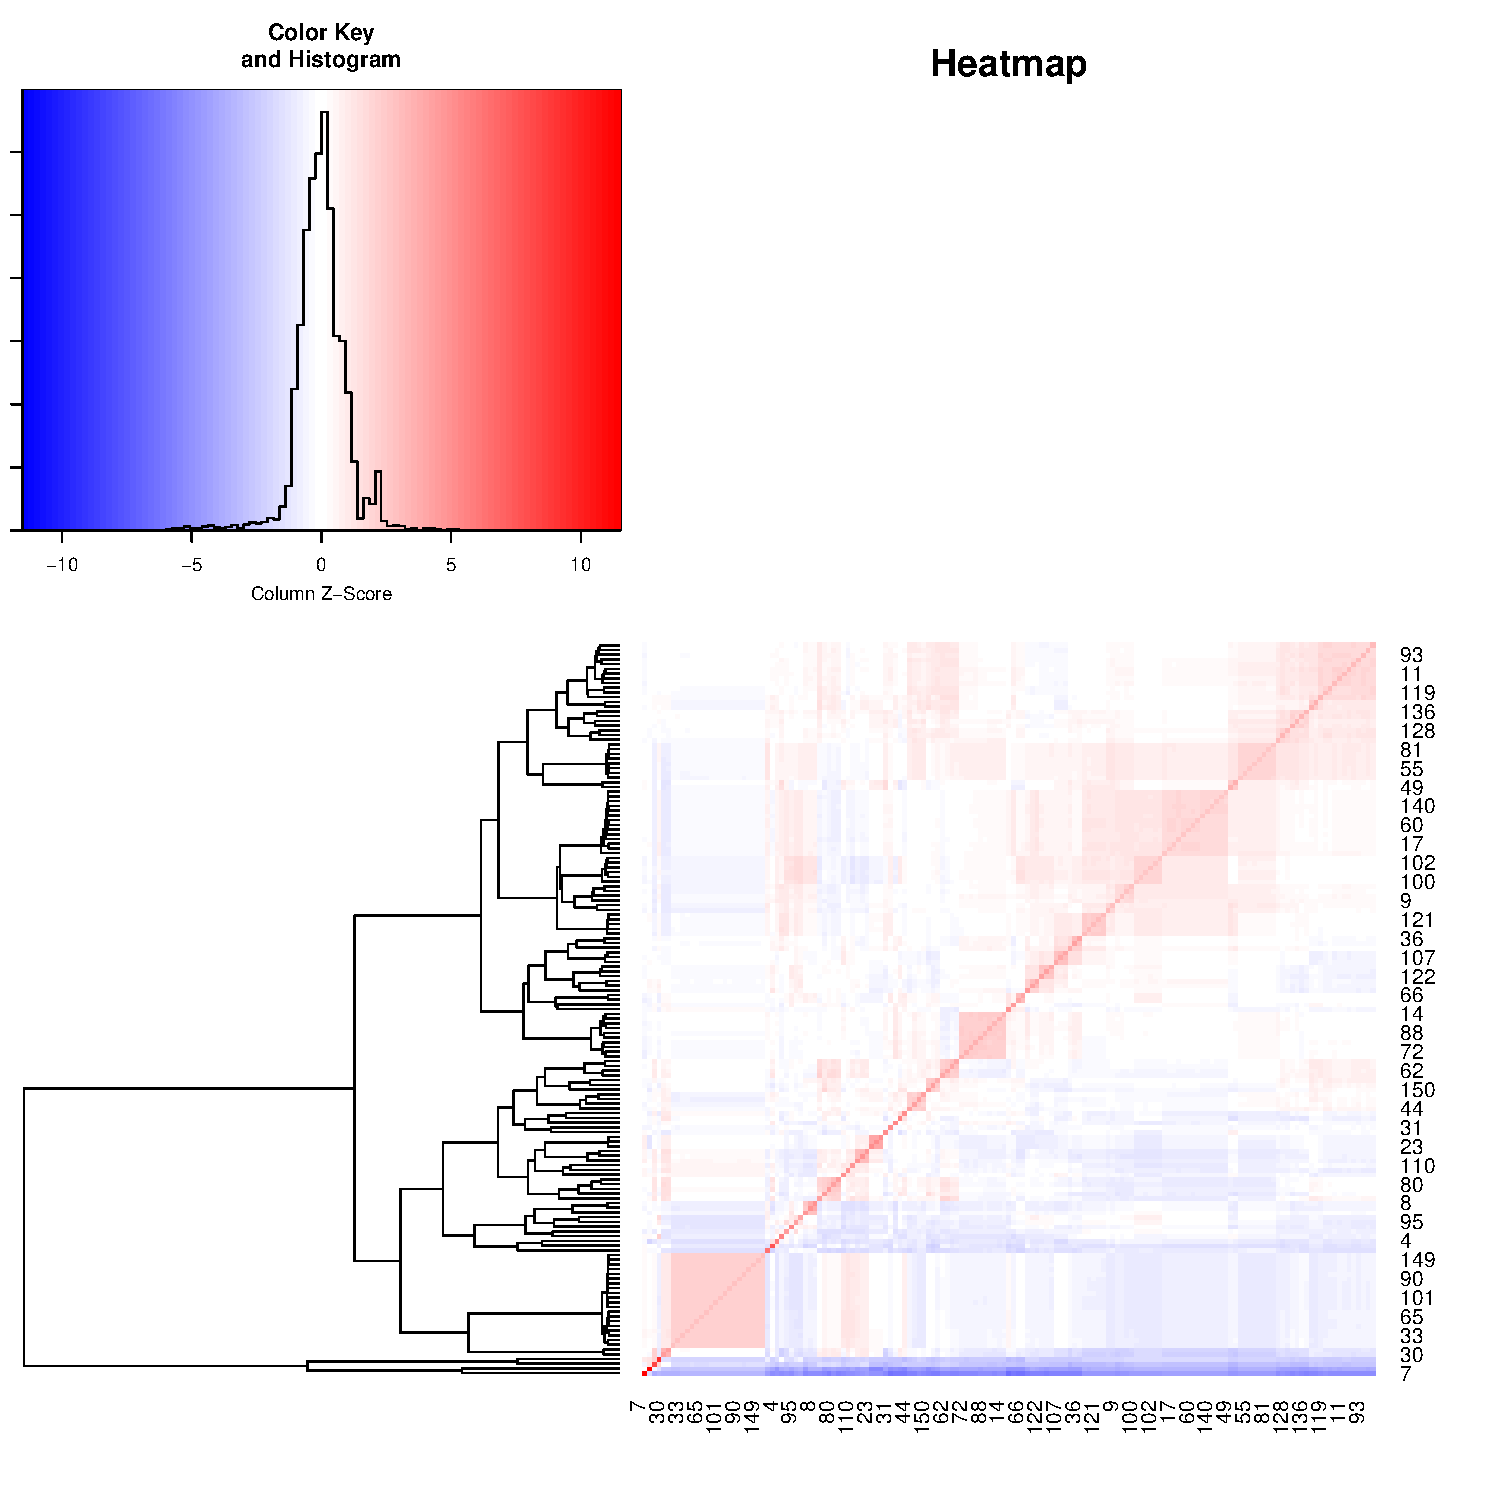
\includegraphics[width=\linewidth]{plot_heatmap.pdf}
\caption{This heatmap includes Altonagård and Ugra soja which are seen as the bottom two blue acessions. They are dissimilar to eachother and dissimmilar to the rest of the accessions.}
\label{fig:heat}
\end{figure}

Characterise genetic relatedness. 
PCA the first 10 pcs capture 22.82\%  of the variation.
the ibs shows identity towards 1 to be at: numbers?

\subsubsection{Distinctness: The SBPA are a genetically cohesive group}
The SBPA are a genetically cohesive group of accessions. In comparison to the CCA, they are similar to each other (matrix numbers?) as seen in the figure the SBPA cluster within the dendrogram of the CCA and the SBPA.  It is also clear that some of the CCA are closely related to the SBPA, which is expected as a domesticated crop and the history known of other pedigrees and breeding programs exchanging germplasm. In the CCA, 94 of the accessions are of European origin and additionally, seven of those  originate from Sweden, some with accession names identical or similar to that of the SBPA. 
\begin{figure}
\centering
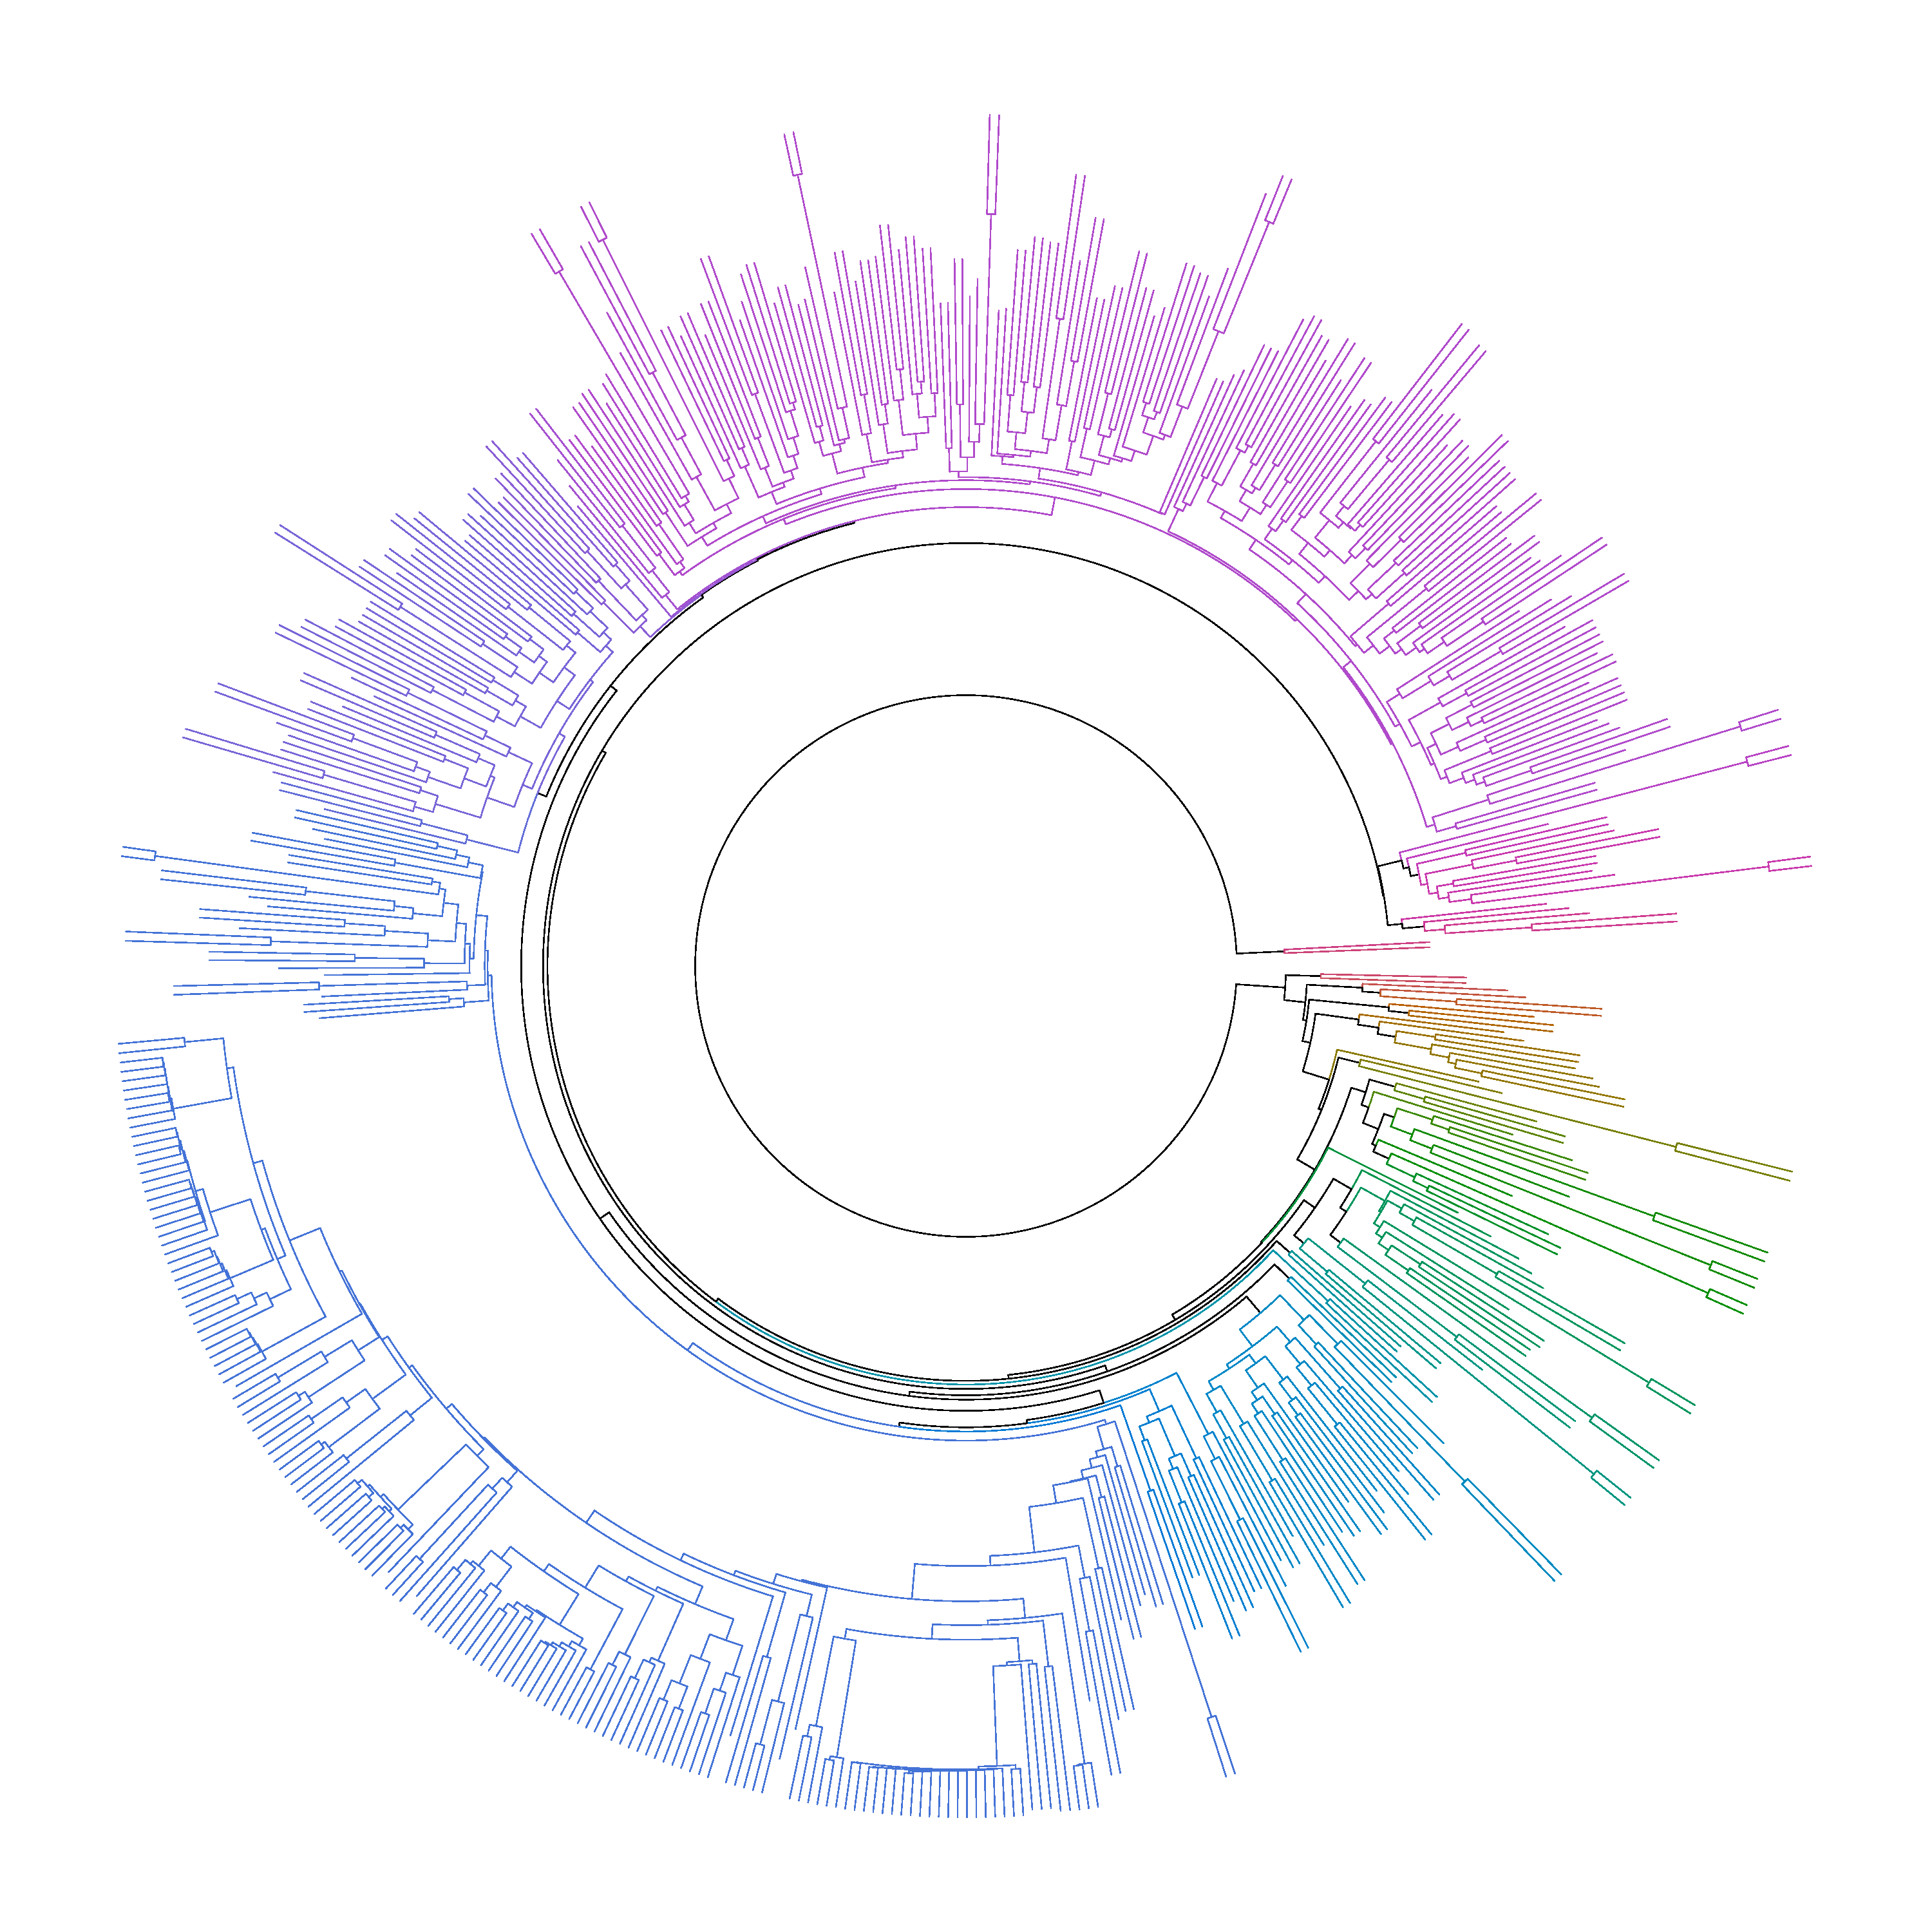
\includegraphics[width=\linewidth]{rainbow.pdf}

\caption{Hierarchical cluster dendrogram based on pairwise identity-by-state (IBS) values from the 50K SNP data for all samples. Including the suspected Founders. The dark blue accessions grouped together are a genetically cohesive group. Based on An IBS analysis is seen that the SBPA are genetically distinct from the other accessions, clustering together. Several Founders are seen clustering hierarchically outside the SBPA. The Swedish accessions Altonagård and Ugra Soja cluster outside }%
\label{fig:dendo}
\end{figure}

\subsubsection{Divergence: There is a (significant) divergence within the subpopulation SBPA of the soybean when comparing other groups of soybean}

Genetic differentiation, e.g., Fst was calculated using SBPA as a subpopulation of the CCA. This is argumentatively valid since the CCA has a variability comparable to the soybean germplasm as a whole (ref). Fst mean at 0.178
The CCA has furthermore been grouped into subpopulations according to Maturation score status to compare the divergence of the SBPA. 
Figure: Fst
The high Fst of the SBPA shows that there is a considerable degree of differentiation in comparison to the other groups defined by maturity group shows 

A relatively high Fst mean between (0.405 \& 0.215) for the SBPA in comparison to the CCA groups shows that there is a considerable degree of differentiation in relation to the other populations as defined by the maturity group. 
The CCA in relation to each other has a relatively low Fst, between (0.075 \& 0.007) showing that differentiation is not high when grouping the CCA by Maturity. 


\textbf{Founders}
p4. summary of what we can see of the founders. 
A list of known and suspected founders has been included in the PCA. It is clear that (some specific) founders are closely related to the SBPA and were clearly founders of the SBP whereas others are not distinguishable as Founders. It is expected that the founder accessions could be more related to accessions in the CCA than the SBPA. A more detailed picture of decent can be seen in the supplementary material where the pedigree data of the SBPA are collected. \nameref{sec:supplementary:material}.

Figure: PCA with founders in. 
The founders could also be indicated earlier in the dendrogram clustering together with the SBPA and the SBPA cluster nested within the founders. 


\subsection{H2 Genetic diversity} 



\textbf{The SBP caused a bottleneck as seen in a decrease in genetic diversity }

There is a reduction of Ne detected in a high level of linkage of the SBPA, the lower nucleotide diversity ($\pi$ ) There is also an accumulation of rare alleles and a lot of alleles fixed in the population. These observations suggest that the bottleneck event and the ensuing intensification of genetic drift had a noticeable impact on the genetic composition of the SBP population.

Earlier studies have shown a halving in nucleotide diversity when comparing wild soybean to their domesticated progenitors and a further halving in nucleotide diversity in breeding regimes in recent years comparing landraces to elite cultivars (ref). The SBPA have a mean nucleotide diversity of ($\pi$ = 0.000999), 0.09\% or a difference of  9/10.000 bases between two sequences. Whereas the CCA has almost double the mean nucleotide diversity of  ($\pi$ = 0.001911)  0.19\% or 19/10.000 bases differing.  The CCA has two times higher nucleotide diversity than the SBPA. This is consistent with a bottleneck during the selection of founders and subsequent selection by the breeding program.  

The nonrandom association of alleles at different sites due to recombination (LD) in soybean shows like in the CCA
In this comparison of CCA and SBPA, we see a high LD at both low and high ranges of the SBPA. The LD slope of the SBPA shows a higher degree of decay over shorter physical distances, indicating in relation to the CCA, a contrasting population size. 

Longer range association estimates a small Ne, because of the bottleneck. 
The long-range LD will be due to a high level of fixation caused by drift.   

figure text:  The LD plot shows the relationship between genetic markers in the two populations at different sites due to recombination. The slope represents the rate at which LD decays with physical distance. The top cyan line is SBPA and the red line is the CCA. 

A difference in slope can also indicate different selective pressures or adaptive processes, such as the steep and higher slope of the SBPA may suggest positive selection or recent selective sweeps. 

AF 
The fixation of alleles due to drift is also seen in the allele frequency of the SBPA. The high number of fixated alleles seen as 
in a high number of allele frequencies in the extremities of the frequency spectrum is a pattern of fixation due to drift. Increased low freq can also be a signal of negative directional selection or a selective sweep, and an increase in high-frequency variants can be a signal of positive directional selection \cite{}. 




\textbf{Allele Frequency shows a high level of drift}
The high number of alleles at high frequency shows that the SBPA have a higher number of monomorphic locus than the CCA. This high number of fixed alleles arises through natural selection, genetic bottlenecks, or genetic isolation in the population. The SBPA also has a large number of rare alleles, a high number of genetic variants in low frequencies. Rare alleles arise through mutation, genetic drift, or migration from other populations. 

The presence of numerous rare alleles, seen in combination with the low pi and high decay, shows the genetic drift in the population. 
or
In conjuncture, the high number of rare alleles and high number of fixed alleles together reveal the bottleneck as also seen in the following LD decay analysis. 

We can deduce this since we know we are not looking at a diverse genetic pool, which could otherwise be a signal of a recent population expansion or balancing selection. Since we conclude that the accumulation of rare alleles is due to drift, we can assume that there is an accumulation of deleterious alleles in a population: The deleterious alleles can arise through spontaneous mutations and random fluctuations in allele frequencies, and the small size of the population leads to an increased frequency of harmful variants.

Although the findings above raise the possibility of potential selection processes occurring in the SBP, the high effect of genetic drift could mask any such signatures of selection making them indistinguishable because the drift enhances random fluctuations in  frequency making it difficult to detect or for the allele to reach fixation.



The next step is to predict if there are areas of the genome where the nucleotide diversity is lower than expected. 

\subsection{H3 Genome-wide selection signatures} 

Selection happened during the Swedish breeding program.
Selection during the Swedish breeding program occurred and can be detected as the accessions are insensitive to photoperiod, and selection occurred signatures are detected at other genomic regions related to seed coat and hilum colour, cold tolerance, and flowering.

Selection at genes of interest.
 Selection can have a similar effect on LD in the genome as a bottleneck can, but it is a localised phenomenon in and around the targeted loci.
We know the breeding program goals and have selected areas to target looking for selection signatures by using areas of the genome that are connected or hypothesised to be relevant to the expression involved to named traits.   
xpclr results. 

haplotype groups? 


The Swedish soybeans are mainly a snapshot of a breeding program stopped around 1978 and all lines or recent crosses from this program were then set into the  







\section{Figures and tables}

\subsection{PCA1 figure}

Figure \ref{fig:pca} shows an example figure.

\begin{figure}[t]
\centering
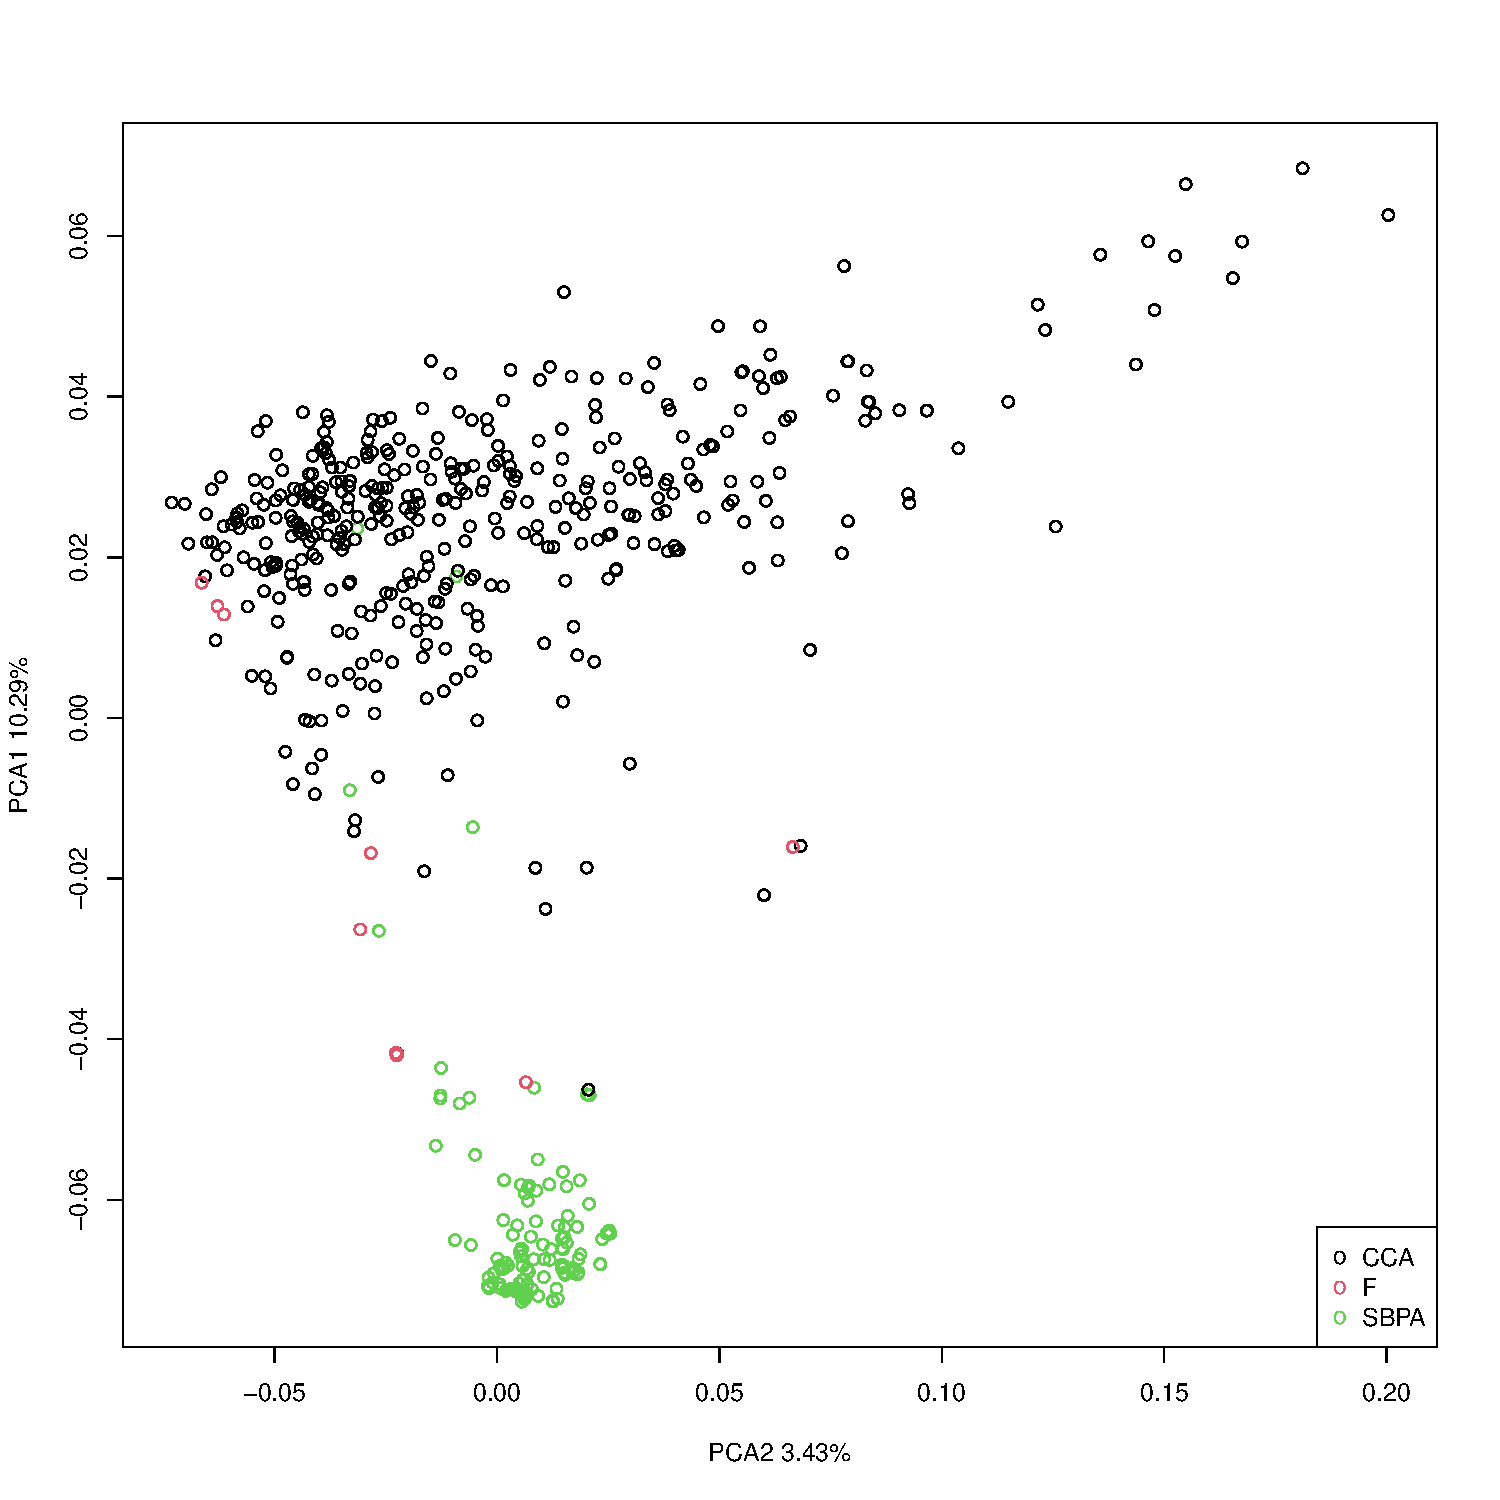
\includegraphics[width=\linewidth]{plot_PCA_source.pdf}
\caption{Biplot of the principal component analysis of soybean genotypes. The colours represent the defined groups; Core collection Accessions (CCA) in black, the Swedish Breeding Program Accessions (SBPA) in green and the Founders of the breeding program (F) in red.}%
\label{fig:pca}
\end{figure}


\subsection{PCA2 figure}


Figure \ref{fig:pca2} .

\begin{figure}[t]
\centering
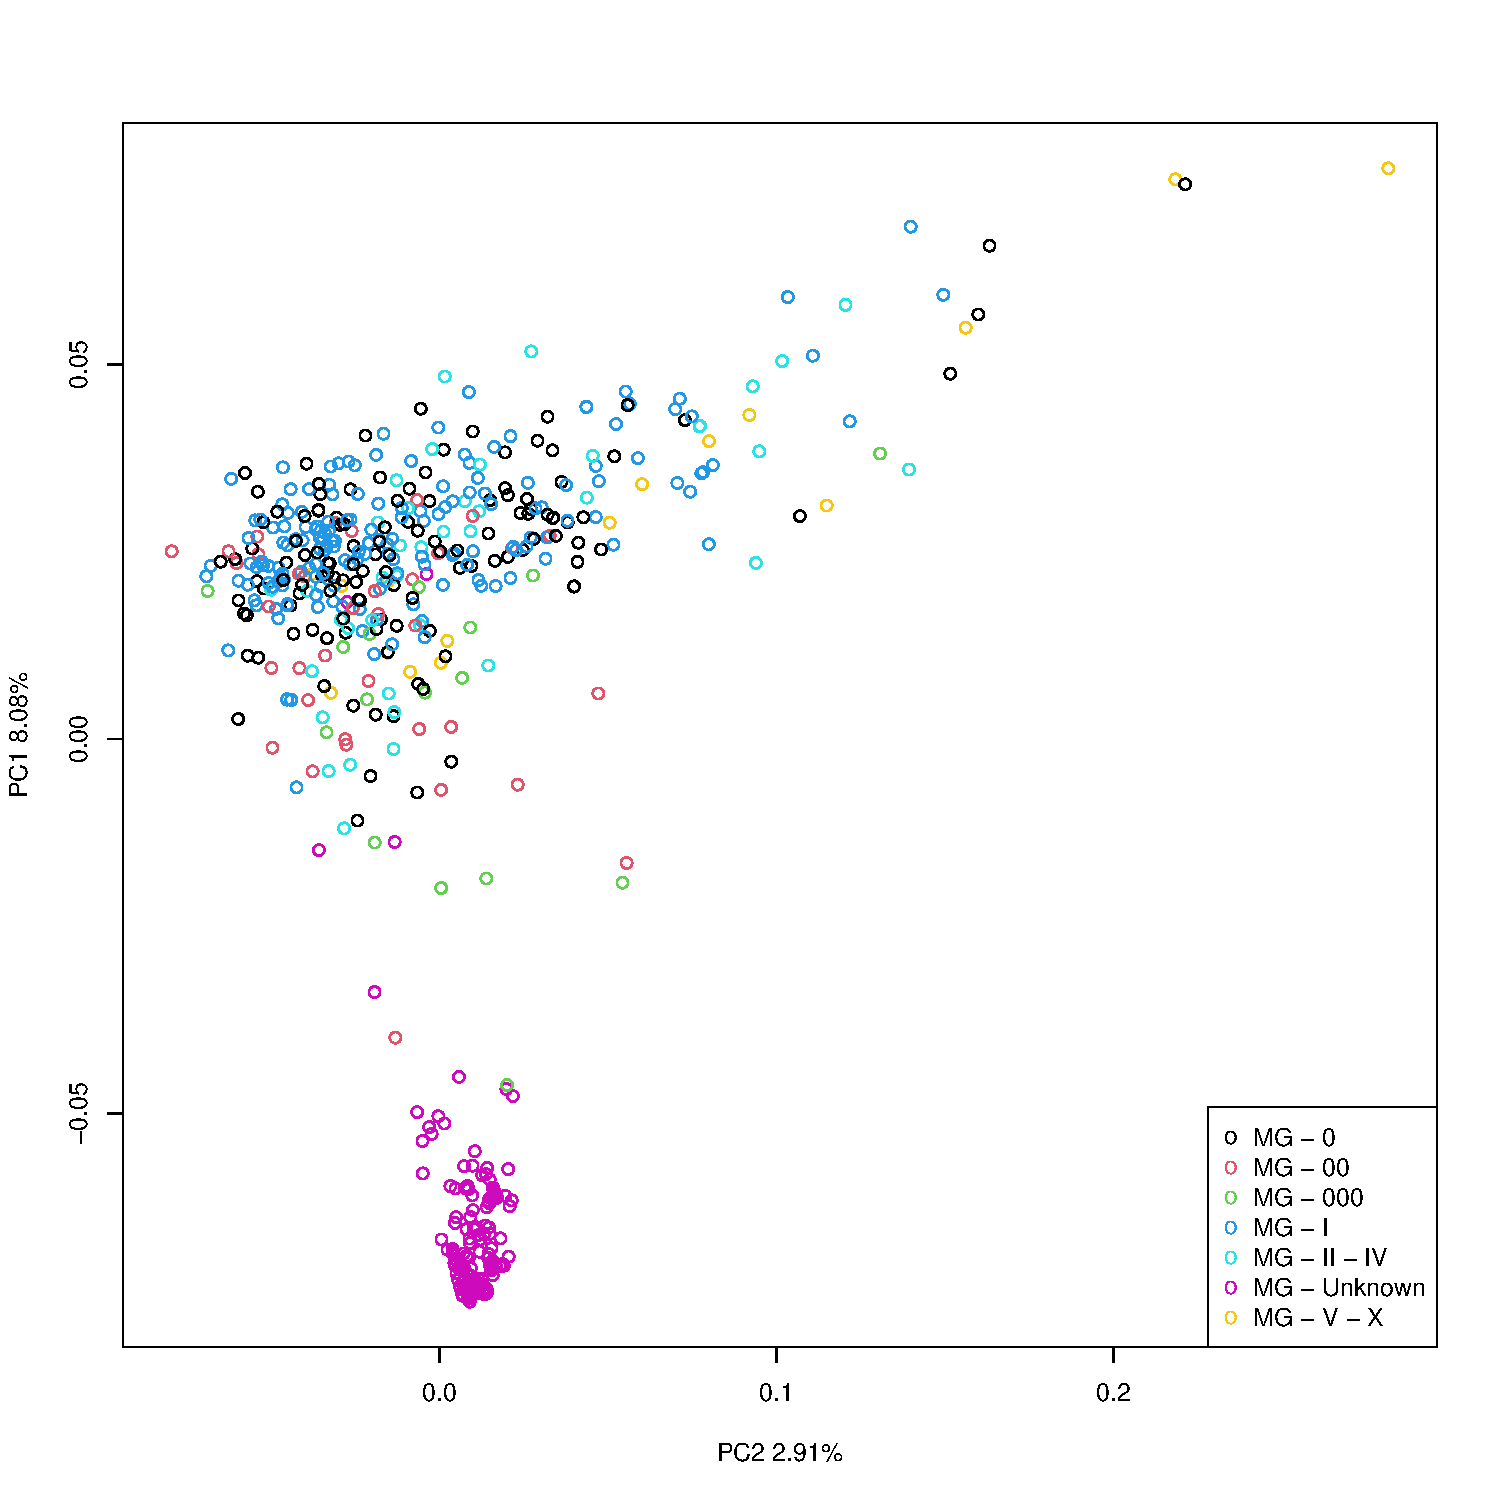
\includegraphics[width=\linewidth]{plot_PCA_mg1.pdf}
\caption{Principal component analysis for soybean samples from the whole genome sequence data, including the 155 Nordgen accessions and the 409 Core collection accessions. Indicated are the Maturity groups assigned to the accessions.}
\label{fig:pca2}
\end{figure}


\subsection{PCA3 figure}


Figure \ref{fig:pca3} .

\begin{figure}[t]
\centering
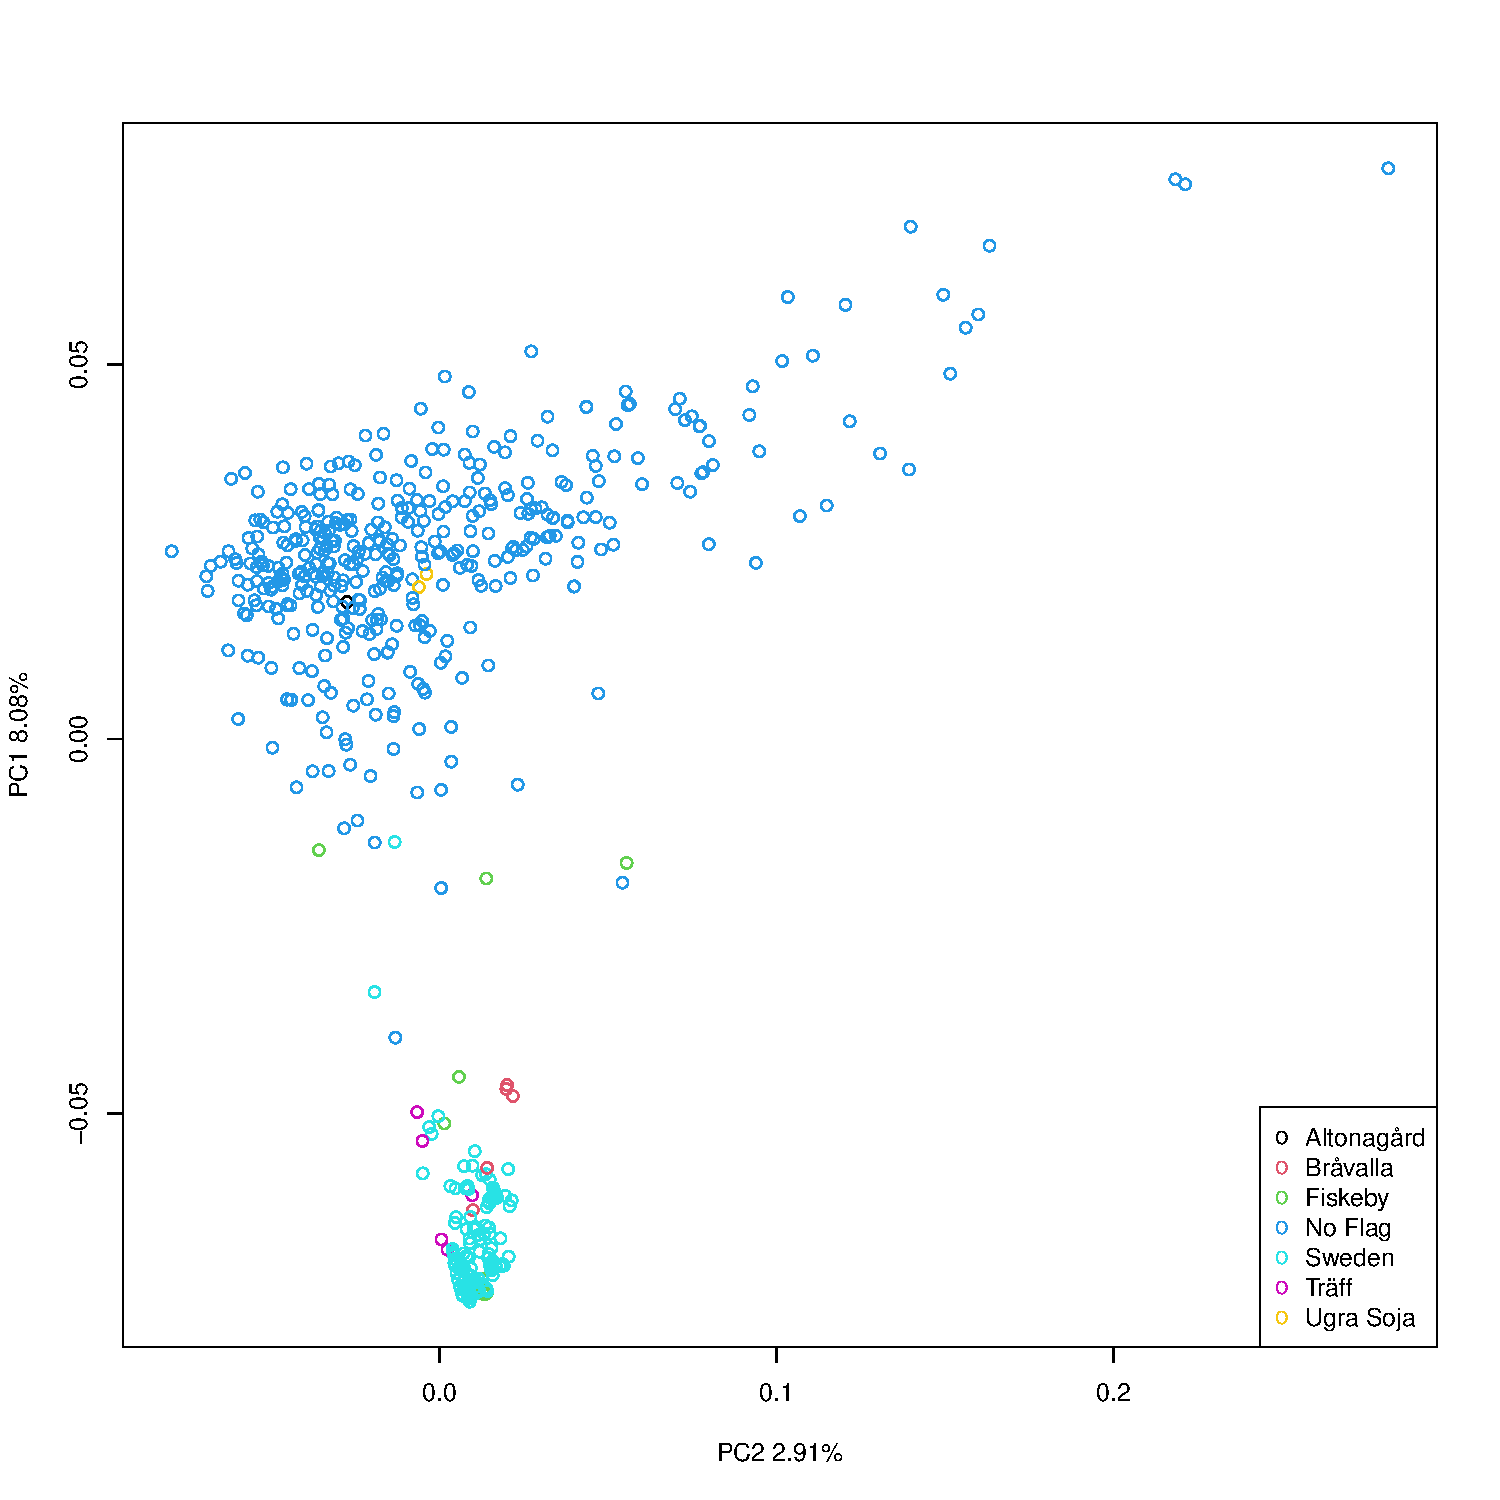
\includegraphics[width=\linewidth]{plot_PCA_flag.pdf}
\caption{PCA flag}
\label{fig:pca3}
\end{figure}



\subsection{PCA figure4}


Figure \ref{fig:pca4} .

\begin{figure}[t]
\centering
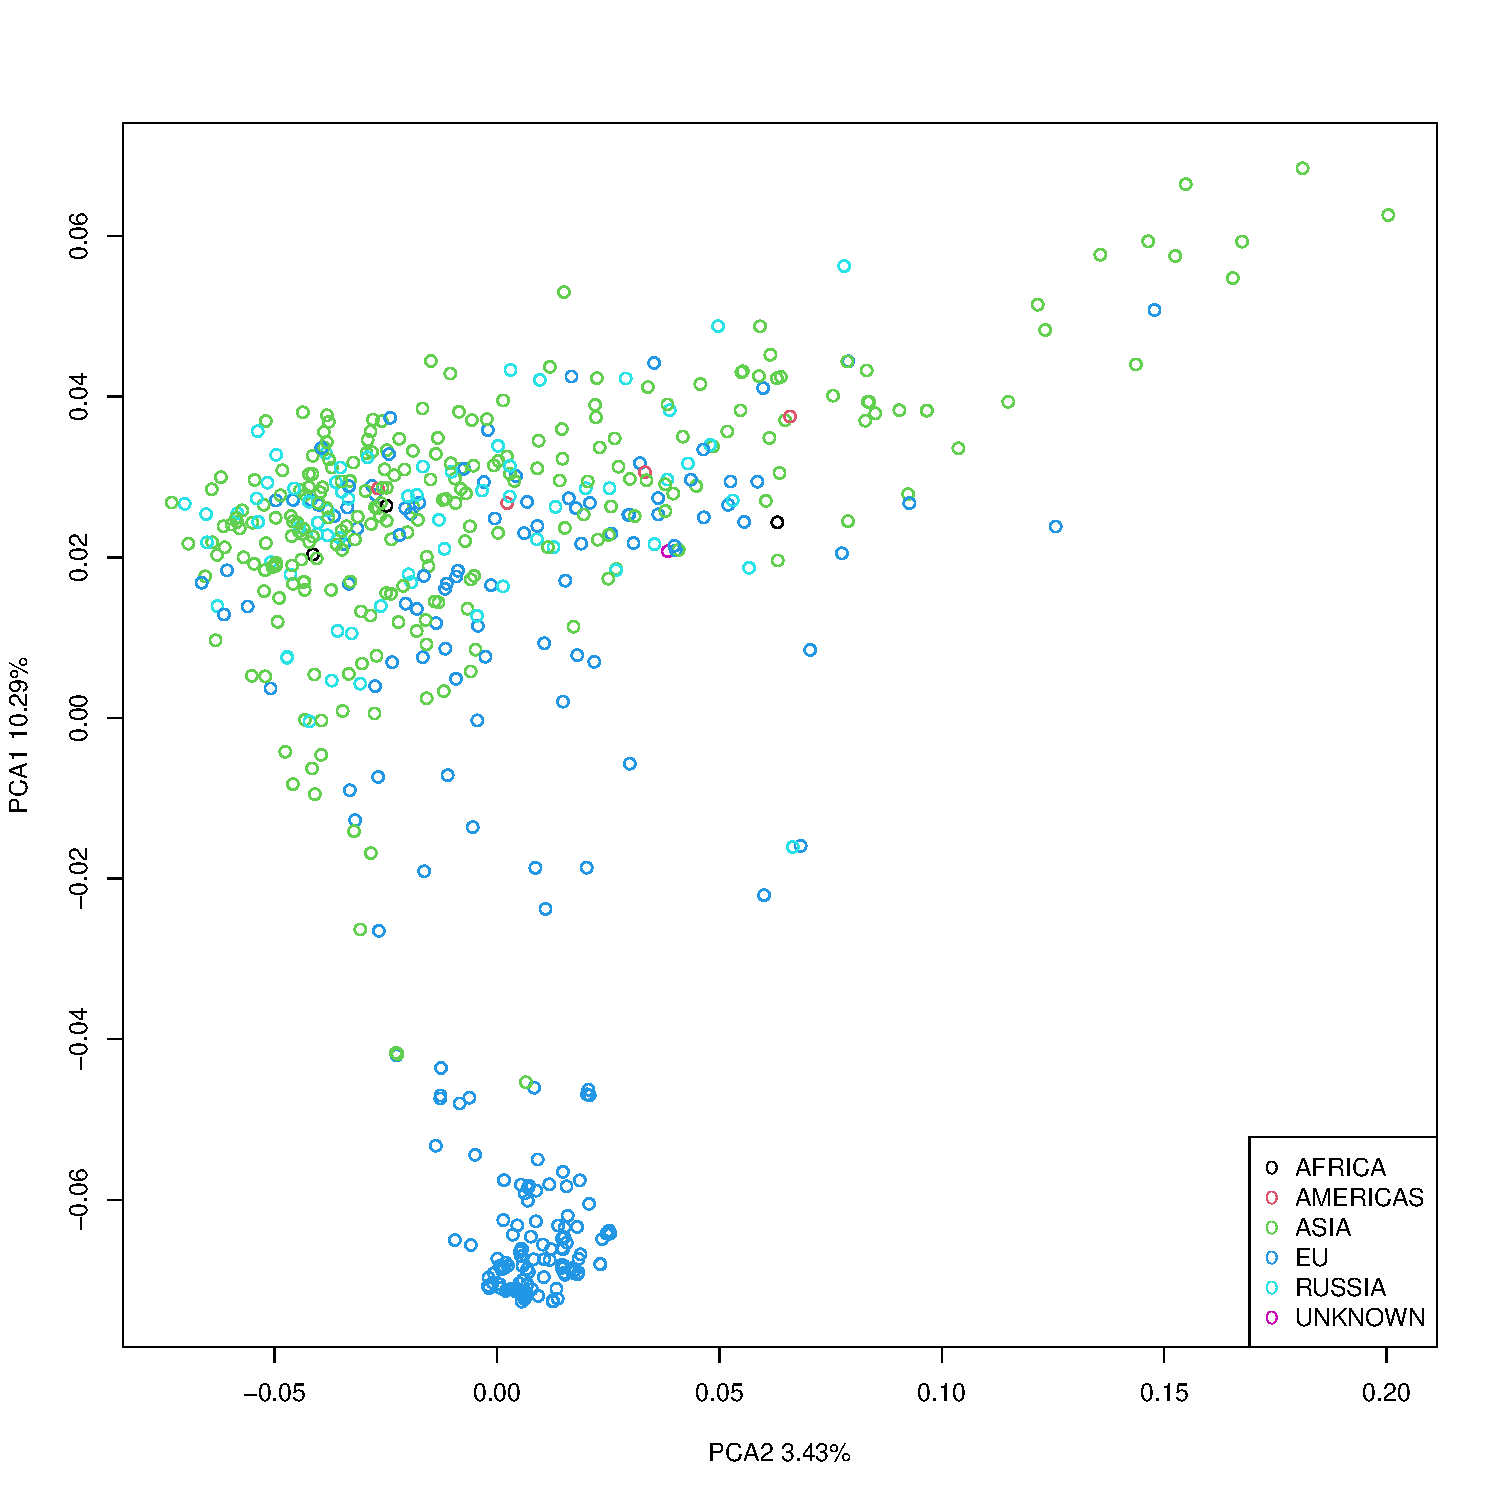
\includegraphics[width=\linewidth]{plot_PCA_region2.pdf}
\caption{PCA regions}
\label{fig:pca4}
\end{figure}


\subsection{Dendogram figure}

Figure \ref{fig:dendo} shows an example figure.

\begin{figure}[t]
\centering
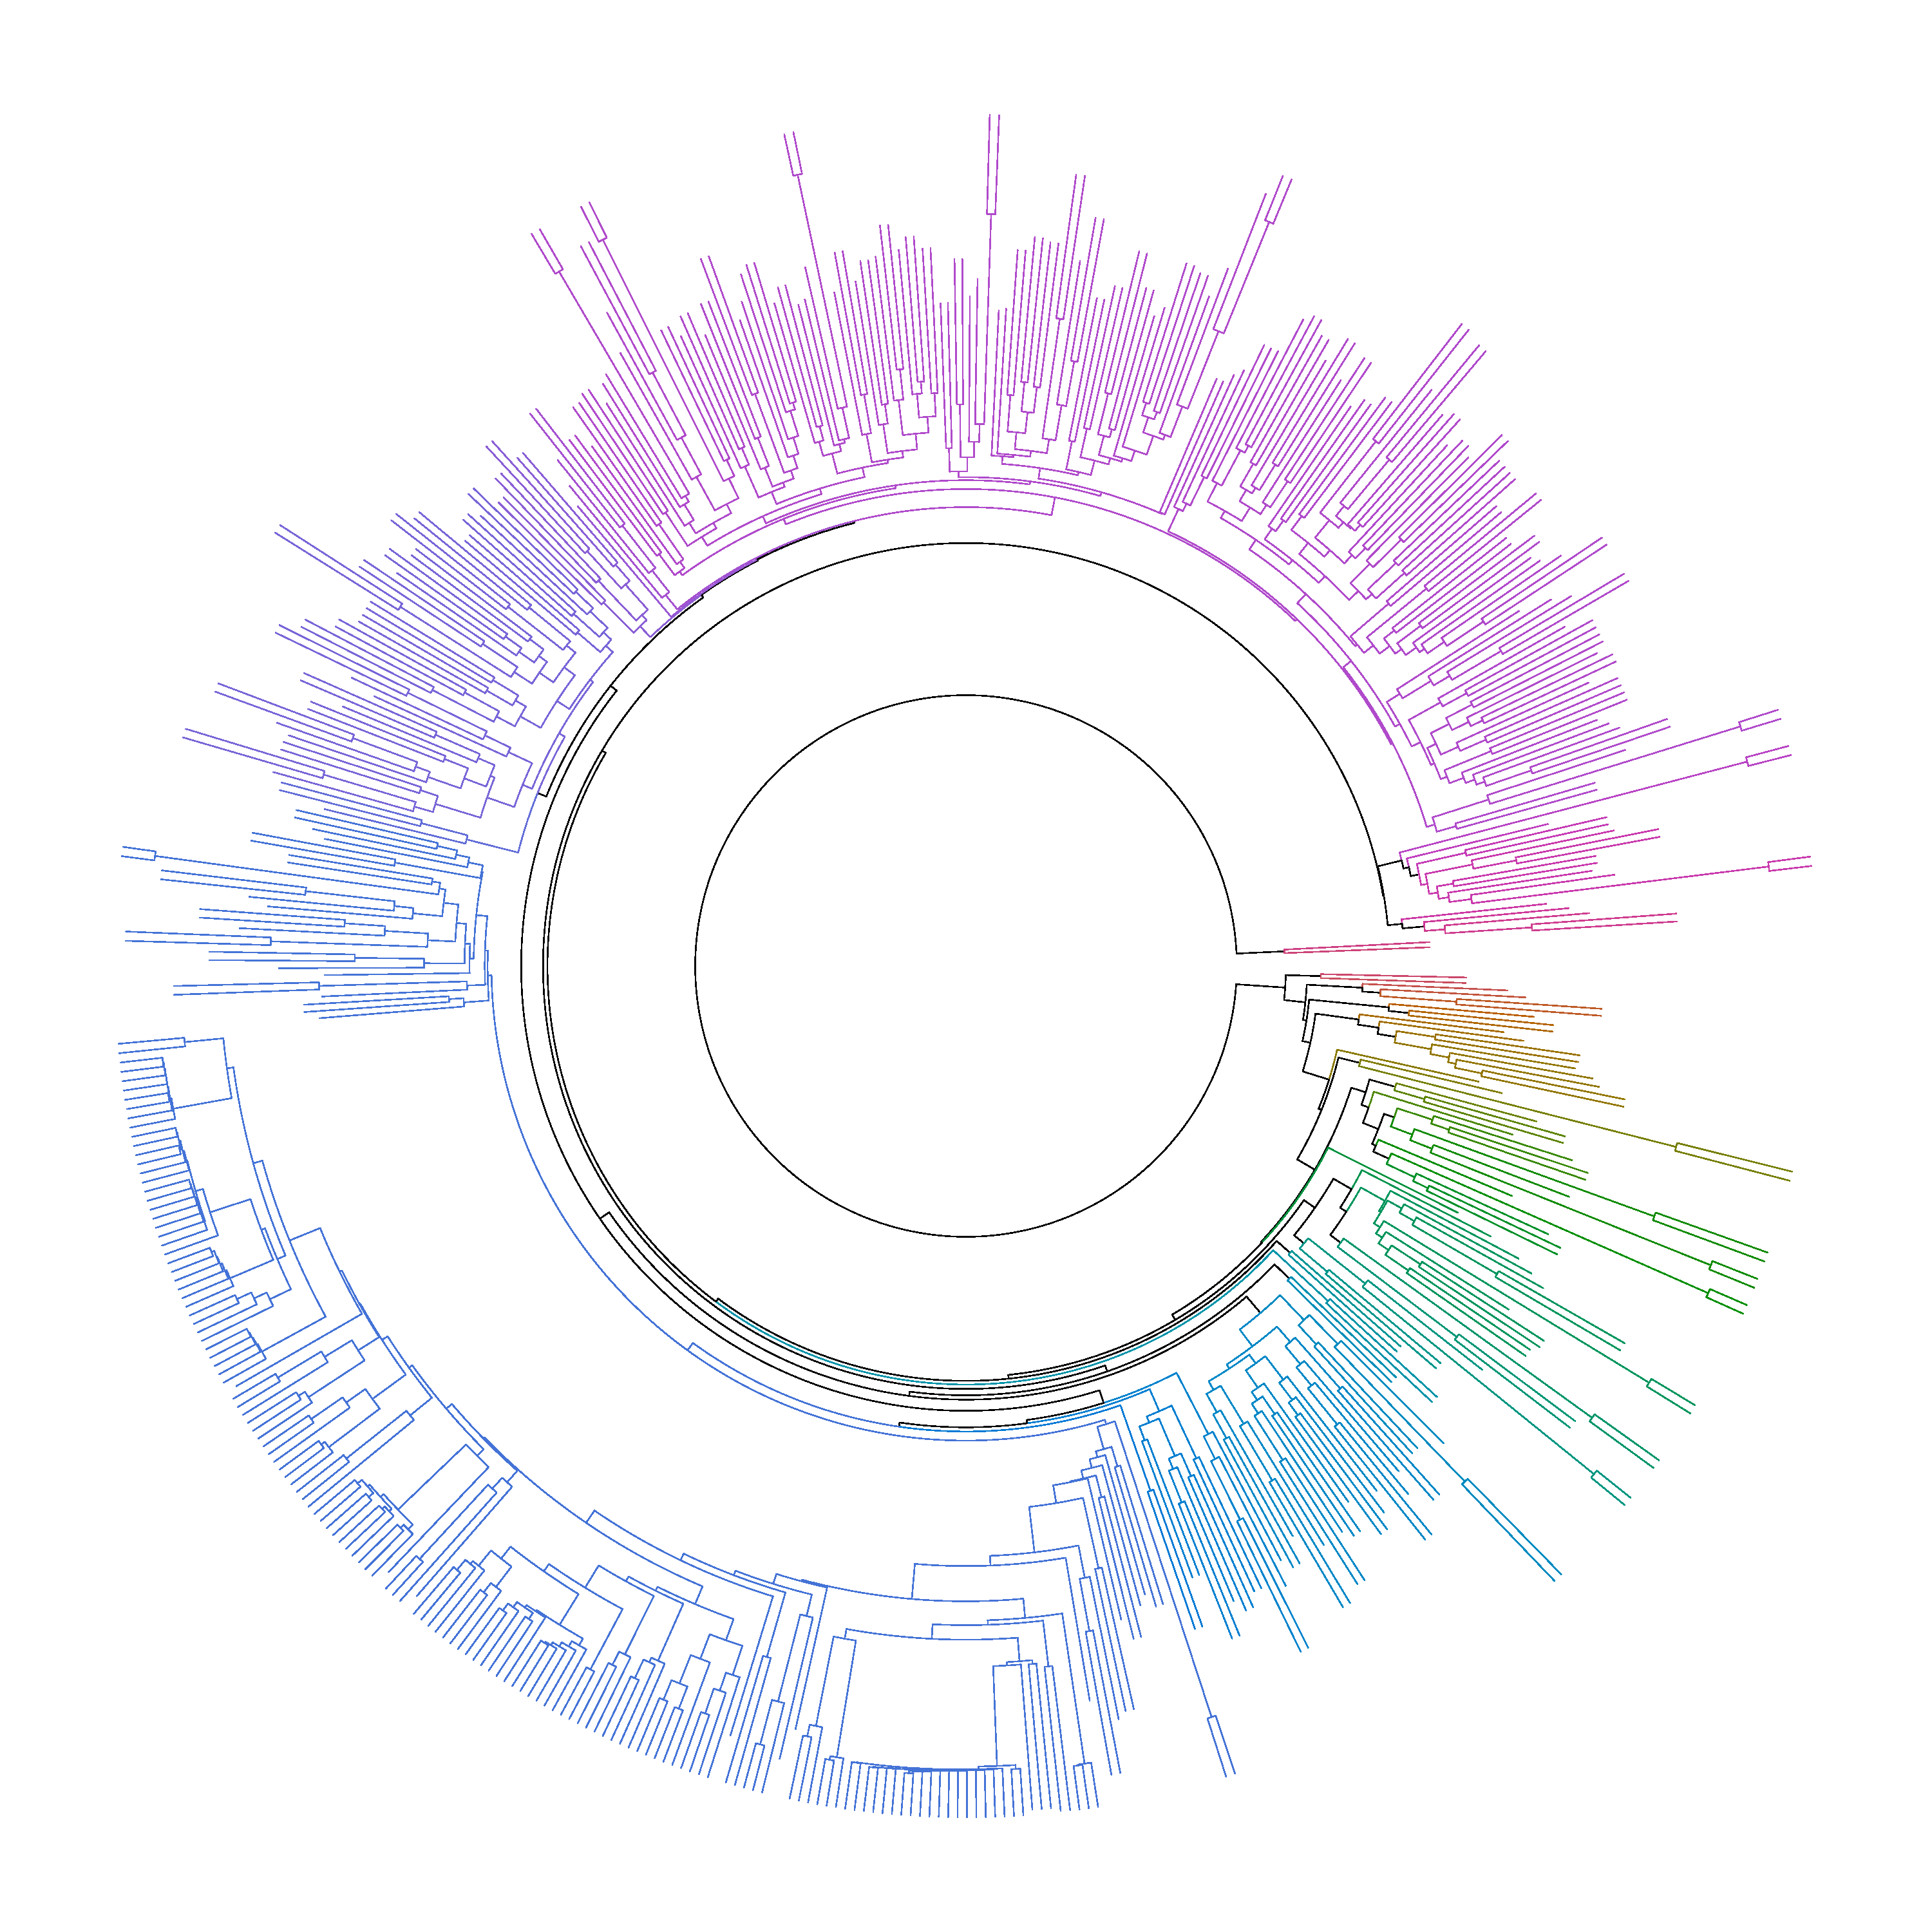
\includegraphics[width=\linewidth]{rainbow.pdf}
\caption{Hierarchical cluster dendrogram based on pairwise identity-by-state (IBS) values from SNP data for all samples. describe dendogram}%
\label{fig:pca}
\end{figure}



\subsection{Heatmap figure}


Figure \ref{fig:heat} .

\begin{figure}[t]
\centering
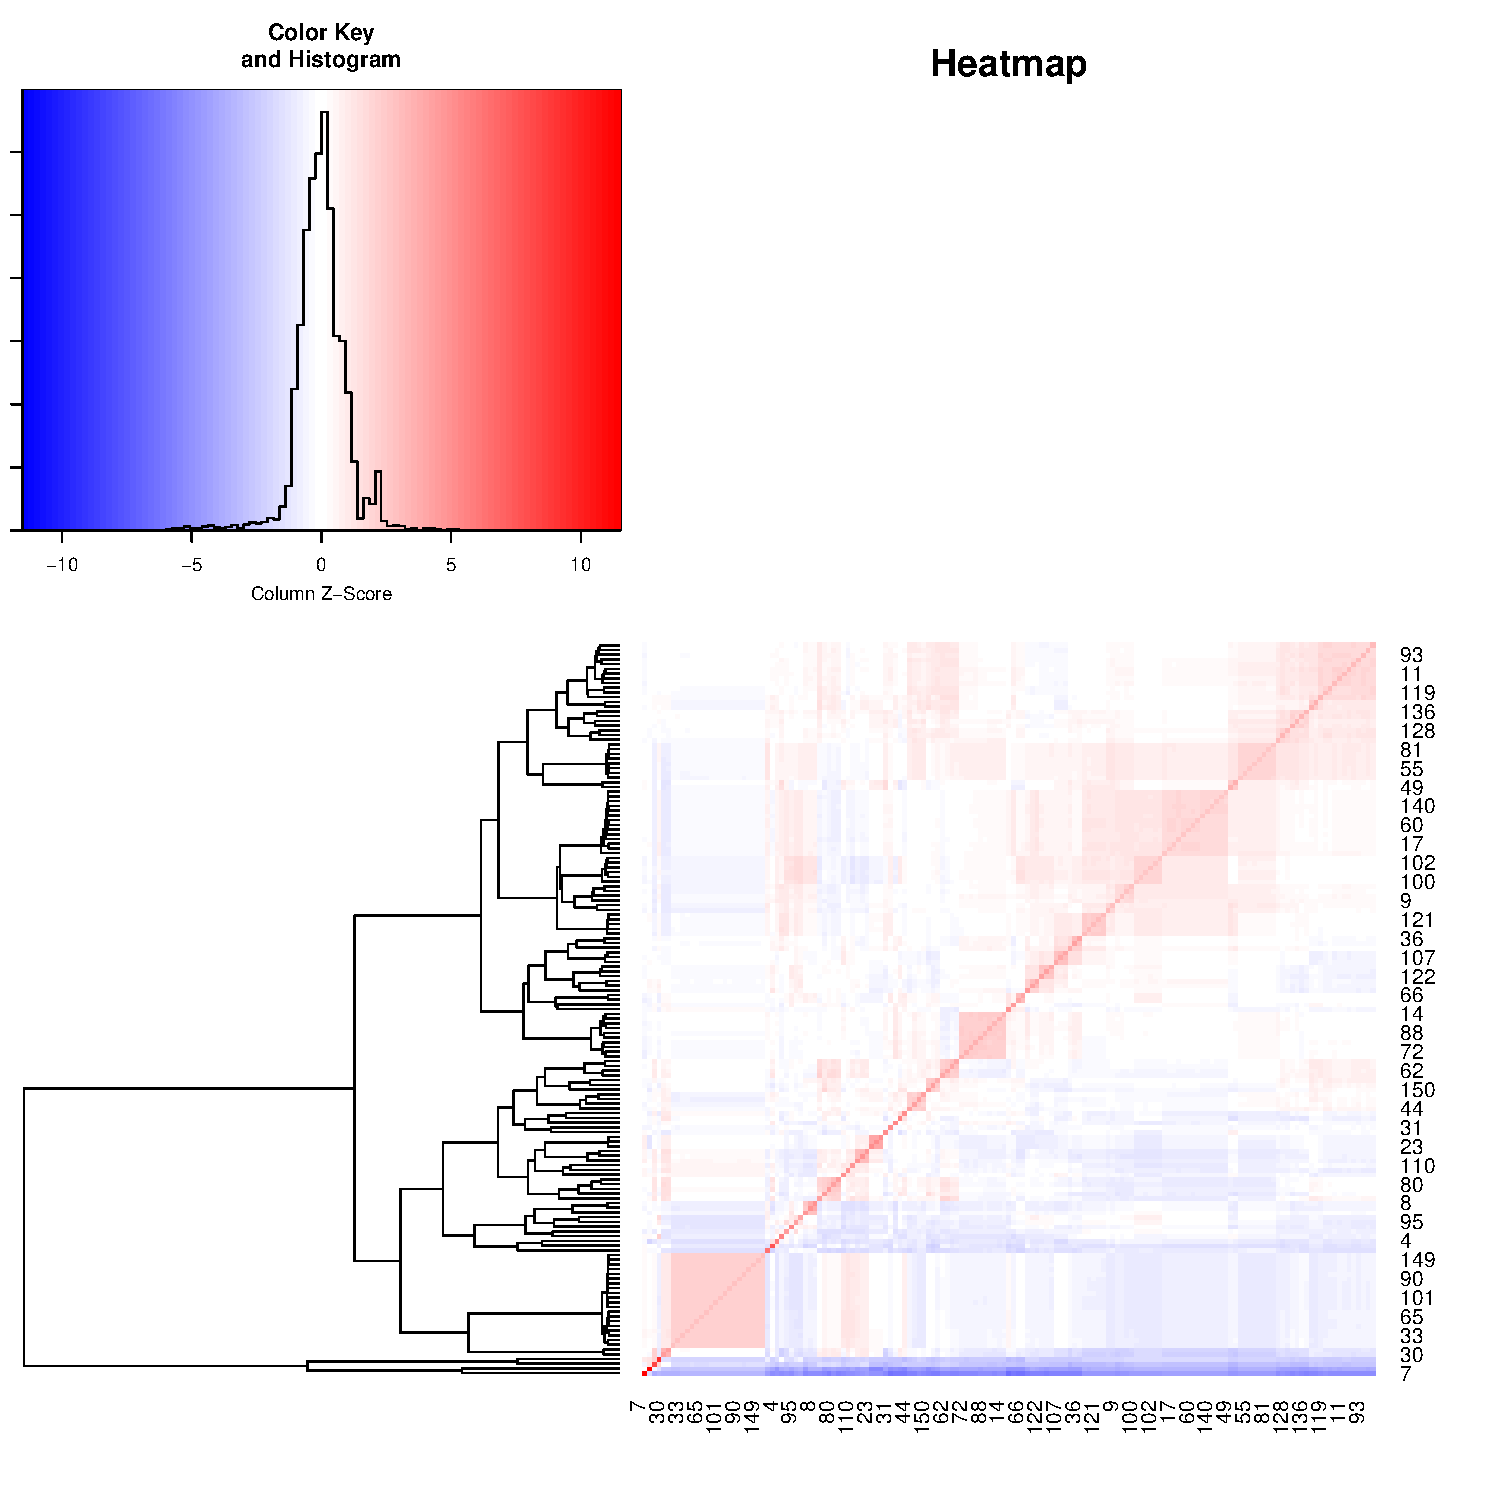
\includegraphics[width=\linewidth]{plot_heatmap.pdf}
\caption{PCA regions}
\label{fig:heat}
\end{figure}



\subsection{Table 1}

Table  \ref{tab:fst} shows table 1. 

\section{other text}

abstract:
Soybean, belonging to the Fabaceae family and scientifically known as \textit{Glycine max} (L. Merrill), is globally recognised as the primary legume crop due to its high protein and oil content. However, its genetic diversity has decreased over time due to domestication and intensive artificial selection, driving the need to look elsewhere to increase germplasm utilisation for abiotic adaptation \citep{hyten06, gizlice96}.  Relevant accessions with the potential for abiotic adaptation to cold tolerance have been identified [@haupt20]. Additionally 160 Swedish accessions, originating from a Swedish breed for the adaptation to the cool climate of north western Europe and stored in the NordGen gene bank have been unearthed [@holmberg1973]. We will interpret the plant genetic resources available, so as to utilise the genetic potential. To facilitate targeted selection of promising accessions from soybeans vast germplasm collections,  and unveiling the genetic data stored in the NordGen seed banks. findings are: ... 


\textbf{Founders}
Founders identified through pedigrees and other genebank metadata have differing similarities to the SBPA. 


\textbf{Ugra soja}
Ugra soja 
"Svalöf’s Ugra soybean is a new variety obtained from a cross between a black-seeded American variety, Wisconsin, and a brown-seeded Polish variety, Brunatna Vilenska. " soybean history book

'Ugra' 
labeled "Ugra", Ugra Saja" & "Ugra Soja"
Developed by Svalöf AB in Malmöhus, Sweden.
Pedigree (Wisconsin Black' with 'Brunatna Vilenska' (a Polish variety).)  It was released in 1950 (source:nordgen).  USDA accession number "Ugra Saja"  is PI 198067 and "Ugra Soja"  at Nordgen NGB 23807

Notes on svalof:

    Svalöf AB later merged with Weibulls AB to form Lantmännen SW seed, a partly Swedish owned seed company. The company is headquartered in Landskrona (Southern Sweden). The town Landskrona is located within the county administration area called Malmö (once called Malmöhus).
    "‘Ugra saja’ is actually just named Ugra. The ‘saja’ is probably just a misspelling of soja (soya in Swedish)." - Dr. Fredrik Fogelberg, Swedish Institute of Agricultural and Environmental Engineering."


\textbf{Altongård}

? Holmberg has been generous in sharing his germplasm with other soybean breeders. Several Canadian workers have used his lines in their crosses. For example, one of the parents of ‘Altona’ is a Holmberg line.?


other text

using the 8 million SNPs of the 409 CCA and 153 SBPA soybeans and the . 

To better understand the population relationships of the accessions received from the Nordic gene bank and how they are related to each other, and the rest of the soybean germplasm, they are here compared to a Core Collection of 409 soybeans from the USDA genebank chosen/curated from the soybean germplasm for Central European breeding.  The Core collection used here is a subset of the soybean germplasm collection, the  USDA genebank accessions, which are assessed to be  preadapted to cultivation in Central Europe, while conserving a high genetic diversity \cite{haupt20}. Additionally, accessions were grouped into categories based on the suspected breeding history.  There are the ten suspected Founders of the Swedish breeding program and the Swedish accessions of the Nordgen genebank. 

A Principal Component Analysis (PCA) and the genome-wide Identity By State (IBS) pairwise distance matrix were applied to visualise the overall variance of the data. The resulting PCA (Figure \ref{fig:pca}) shows the clustering of the Swedish accessions as a sub-group based on similarity. The variance proportions explained. 

A closer look at the PCA revealed two accessions of the Nordgen Swedish that were not part of the particular breeding program of interest as seen in (Figure \ref{fig:pca3}  showing the PCA indicating the two accessions not from the breeding program in the cluster with the CCA in orange and black)  and also thereafter confirmed by the genebank passport data that they originated from other Swedish soybean breeding programs (mention more here when certain. Altonagård and Ugra soja/ saja, malmåhus).  This figure also shows the accessions of the Nordgen and core collection that are Swedish of origin and with a name consisting of letters (excluding numbers or non-alphanumeric characters of the accessions' names) as included in the database. 
The IBS (Figure  \ref{fig:dendo}) clearly shows the Swedish accessions of the breeding program of interest clustering together. The  
 IBS numbers in a table showing ibs within sbpa and out?

 Heatmap based on the sbpa shows high similarity of the SBPA and shows that the 2 accessions Altonagård/Altonagard and Ugra Soja(Saja) are dissimilar. 

The population differentiation measured by $F_{\text{ST}}$
i think we agreed that we needed 

change values:
Fst estimation on genotypes:
Excluding 0 SNP (monomorphic: TRUE, MAF: NaN, missing rate: NaN)
    # of samples: 564
    # of SNPs: 8,533,444
Method: Weir & Hill, 2002
### of Populations: 2
    CCA (409), SBPA (155)
[1] 0.2412619
[1] 0.1783931
     Min.   1st Qu.    Median      Mean   3rd Qu.      Max. 
-0.002281  0.048690  0.136954  0.178393  0.263807  0.938701 
\begin{table}[p]
\centering 
\caption{$F_{\text{ST}}$ estimation on genotypes. Measuring the population differentiation of  the 155 Accessions of the Nordgen genebank (Do again with only the 153 that were part of the breeding program)(SBPA) to the Core Collection of 409 accessions (CCA).}

\begin{tableminipage}{\textwidth}
\begin{tabular}{|l|l|l|l|l|l|l|}
\hline

Samples:                        &564        &          &          &          &          &          \\ \hline
SNPs:                           & 8,533,444 &          &          &          &          &          \\ \hline
Method: Weir \& Cockerham, 1984 &           &          &          &          &          &          \\ \hline
Populations:                  & CCA       & 409      & SBPA     & 155      &          &          \\ \hline
Weighted Fst estimate:          &0.2231884  &          &          &          &          &          \\ \hline
Mean Fst:                       &0.1108533  &          &          &          &          &          \\ \hline
summary:                        & Min.      & 1st Qu   & Median   & Mean     & 3rd Qu.  & Max.     \\ \hline
                                & -0.002515 & 0.011669 & 0.041730 & 0.110853 & 0.145697 & 0.975485 \\ \hline
\end{tabular}
  \label{tab:fst}
\end{tableminipage}
\end{table}


\begin{figure}
    \centering
    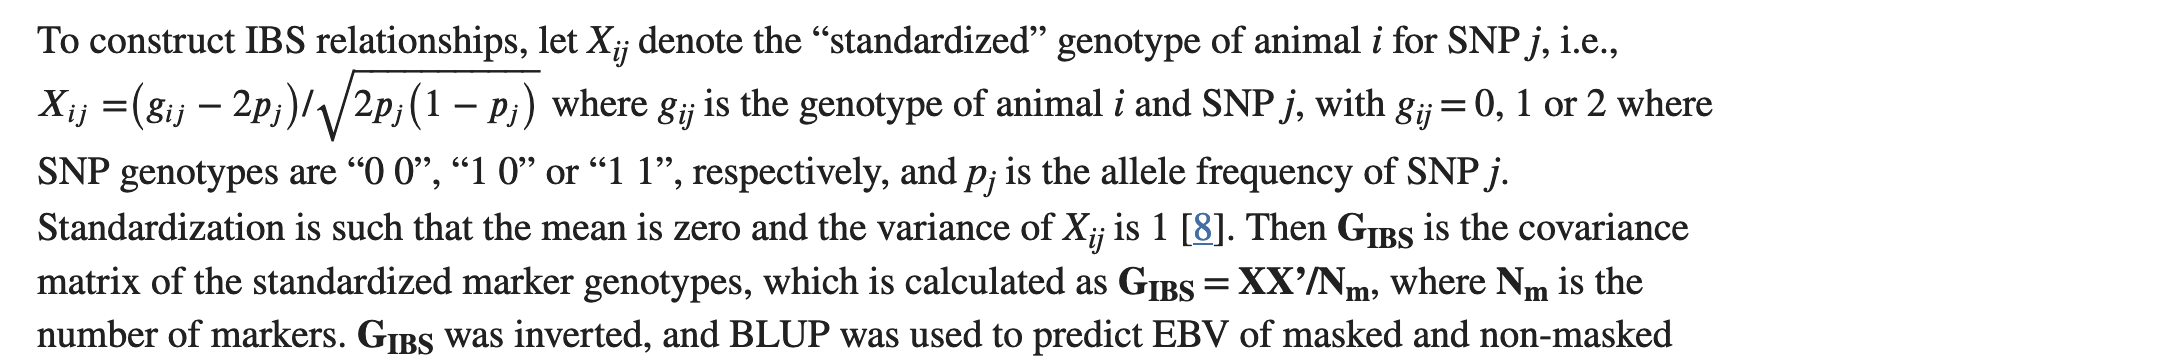
\includegraphics[width=0.5\linewidth]{Screenshot 2023-07-02 at 14.40.39.png}
    \caption{https://www.ncbi.nlm.nih.gov/pmc/articles/PMC3517337/}
    \label{fig:enter-label}
\end{figure}




\begin{table}[p]
\centering 
\caption{$F_{\text{ST}}$ estimation on Maturity groups, measuring the population differentiation of  the 155 Accessions of the Nordgen genebank that were part of the breeding program)(SBPA) to the Core Collection of 409 accessions (CCA) groups by the corosponding maturist groups.}

\begin{tableminipage}{\textwidth}
\begin{tabular}{|l|c|l|l|l|l|l|l|l|l}
\cline{1-9}
\multicolumn{1}{|c|}{\begin{tabular}[c]{@{}c@{}}Weir and Cockerham \\ mean Fst estimate\end{tabular}} &                & Group 1                                       & Group 2                           & Group 3                           & Group 4                           & Group 5                           & Group 6                           & Group 7                    &  \\ \cline{1-9}
                                                                                                      & Maturity group & \multicolumn{1}{c|}{SBPA}\footnote{The Maturity Group of the SBPA are not known and grouped in one group.}\\                     & \multicolumn{1}{c|}{0-0-0}        & \multicolumn{1}{c|}{0-0}          & \multicolumn{1}{c|}{0}            & \multicolumn{1}{c|}{I}            & \multicolumn{1}{c|}{II - IV}      & \multicolumn{1}{c|}{V - X} &  \\ \cline{1-9}
Group 1                                                                                               & SBPA           & \multicolumn{1}{c|}{\cellcolor[HTML]{E7E6E6}} & \cellcolor[HTML]{E7E6E6}          & \cellcolor[HTML]{E7E6E6}          & \cellcolor[HTML]{E7E6E6}          & \cellcolor[HTML]{E7E6E6}          & \cellcolor[HTML]{E7E6E6}          & \cellcolor[HTML]{E7E6E6}   &  \\ \cline{1-9}
Group 2                                                                                               & 0-0-0          & \cellcolor[HTML]{93CC7E}0.2968376             & \cellcolor[HTML]{E7E6E6}          & \cellcolor[HTML]{E7E6E6}          & \cellcolor[HTML]{E7E6E6}          & \cellcolor[HTML]{E7E6E6}          & \cellcolor[HTML]{E7E6E6}          & \cellcolor[HTML]{E7E6E6}   &  \\ \cline{1-9}
Group 3                                                                                               & 0-0            & \cellcolor[HTML]{9FD07F}0.2702235             & \cellcolor[HTML]{FBAB77}0.0306470 & \cellcolor[HTML]{E7E6E6}          & \cellcolor[HTML]{E7E6E6}          & \cellcolor[HTML]{E7E6E6}          & \cellcolor[HTML]{E7E6E6}          & \cellcolor[HTML]{E7E6E6}   &  \\ \cline{1-9}
Group 4                                                                                               & 0              & \cellcolor[HTML]{B5D680}0.2212166             & \cellcolor[HTML]{FDCD7E}0.0428267 & \cellcolor[HTML]{F98B71}0.0191540 & \cellcolor[HTML]{E7E6E6}          & \cellcolor[HTML]{E7E6E6}          & \cellcolor[HTML]{E7E6E6}          & \cellcolor[HTML]{E7E6E6}   &  \\ \cline{1-9}
Group 5                                                                                               & I              & \cellcolor[HTML]{B8D780}0.2146631             & \cellcolor[HTML]{FEE983}0.0525354 & \cellcolor[HTML]{FA9D75}0.0255972 & \cellcolor[HTML]{F8696B}0.0068046 & \cellcolor[HTML]{E7E6E6}          & \cellcolor[HTML]{E7E6E6}          & \cellcolor[HTML]{E7E6E6}   &  \\ \cline{1-9}
Group 6                                                                                               & II - IV        & \cellcolor[HTML]{8FCB7E}0.3063683             & \cellcolor[HTML]{FFEB84}0.0532384 & \cellcolor[HTML]{FCC27C}0.0387984 & \cellcolor[HTML]{FBA576}0.0282634 & \cellcolor[HTML]{FA9172}0.0212429 & \cellcolor[HTML]{E7E6E6}          & \cellcolor[HTML]{E7E6E6}   &  \\ \cline{1-9}
Group 7                                                                                               & V - X          & \cellcolor[HTML]{63BE7B}0.4046471             & \cellcolor[HTML]{F6E984}0.0745305 & \cellcolor[HTML]{F7E984}0.0728984 & \cellcolor[HTML]{FCEB84}0.0607337 & \cellcolor[HTML]{FFEB84}0.0548296 & \cellcolor[HTML]{FBAA77}0.0301916 & \cellcolor[HTML]{E7E6E6}   &  \\ \cline{1-9}
\end{tabular}
  \label{tab:fst2}
\end{tableminipage}
\end{table}


postulate: Population subdivision analysis will quantify the SPBA will be a distinct subpopulation with a moderate to distinct allele frequency difference.

\section{Supplementary Material}
\label{sec:supplementary:material}

(S1: Overview) Detailed descriptions of all supplemental files. 
(S2: Accessions) Accession and pedigree data 
(S3: Methods 1) data preparation and filtering 
(S4: Methods 3) data analysis
(S5: Results)
(S6: Historical) Supplementary material historical information 

\subsection{Description of Supplementary Material}
File S1 contains detailed descriptions of all supplemental files. 
File S2 contains SNP ID numbers and locations. File S3 contains genotypes for each individual. Sequence data are available at GenBank and the accession numbers are listed in File S3. Gene expression data are available at GEO with the accession number: GDS1234. 

\section{Data availability}
\label{sec:data:availability}
For example: genotype data wgs are available upon request? 
File S1 contains detailed descriptions of all supplemental files. File S2 contains SNP ID numbers and locations. File S3 contains genotypes for each individual. Sequence data are available at GenBank and the accession numbers are listed in File S3. Gene expression data are available at GEO with the accession number: GDS1234. 
All code can be found at \url{https://github.com/JosephineConnelly/soyadapt_data_analysis}.

\section{Acknowledgments}
Acknowledgments should be included here.

\section{Funding}
Funding, including Funder Names and Grant numbers should be included here.

\section{Conflicts of interest}
There are  no known conflicts of interest.

## 
## To cite R in publications use:
## 
##   R Core Team (2021). R: A language and environment for statistical
##   computing. R Foundation for Statistical Computing, Vienna, Austria.
##   URL https://www.R-project.org/.
## 
## A BibTeX entry for LaTeX users is
## 
##   @Manual{,
##     title = {R: A Language and Environment for Statistical Computing},
##     author = {{R Core Team}},
##     organization = {R Foundation for Statistical Computing},
##     address = {Vienna, Austria},
##     year = {2021},
##     url = {https://www.R-project.org/},
##   }
## 
## We have invested a lot of time and effort in creating R, please cite it
## when using it for data analysis. See also 'citation("pkgname")' for
## citing R packages.

\bibliography{bibliography}

    To insert a bibliography where bibfilename is the name of a .bib file.

\bibliographystyle{genetics}

        To choose a BibTeX bibliographic style file with the extension .bst.


\end{document} 